\section{Implementation of the Dynamic Honeycomb Maze}
\label{section:implementation}
The design of this maze has three basic interacting units.
They are:
\begin{enumerate}
    \item The \textbf{\textit{Animal}}, which makes a decision about which platform it would like to move to.
    \item The \textbf{\textit{Robot}s}, which move around the grid as required to provide the animal further movement choices for the animals path.
    % \item The \textbf{\textit{Maze}}, which is the set of all points in the grid within which the robots can navigate around in.
    \item The \textbf{\textit{Maze}}, which is the hexagonal grid comprised of the positions upon which the robots can navigate around on.
\end{enumerate}

% \begin{figure}[h]
%     \centering
%     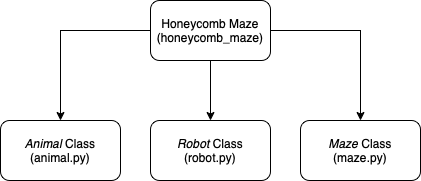
\includegraphics[scale= 0.5]{images/structure.png}
%     \caption{Structure of the Program}
%     \label{fig:my_label}
% \end{figure}

As such the program has been structured into these three blueprints of the objects involved, known as a '\textit{class}' in object oriented programming; relevant functions are placed into the relevant classes.

\subsubsection{\textit{Inner Ring}, \textit{Outer Ring} and \textit{Relative Position}}

% Because of the importance of these two ideas in the development of this algorithm these two ideas have been introduced before the explanation of where they are used in the algorithm.

% The movement of the robots occur in relation to each-other, for example 'a movement \textit{away} from another robot' or '\textit{around} each other'. As such  these relative heuristics are developed for computing the robots' place in relation to each-other and are used in many parts of the program to compute moves.

The robots are always moving in relation to each-other. Therefore metrics of 'relation' have been to be developed. The robots positional relationship has to be computed in order to dictate decisions and potential movements \textit{relative to each-other} in many places in the program.

These two important heuristics of relation have been developed to compute their relationship between the robots in the Honeycomb Maze.

\paragraph{Inner and Outer Ring}

The \textit{inner ring} is the set of 6 hexagonal tiles that are adjacent to one central tile. These are the orange tiles in Fig \ref{fig:inner_ring}.
The \textit{outer ring} are the set of 12 tiles that are all exactly 2 moves away from the central tile (blue tiles in Fig \ref{fig:inner_ring})
Often the inner and outer ring will be computed from the robot occupied by the animal (as shown in Fig \ref{fig:inner_ring}). See function \ref{function:def_inner_ring} for implementation.

\paragraph{Relative position}

Relative position acts as a mapping of all of the six hexagonal points on the inner ring (labeled 'a') to points on the outer ring (labeled 'b') where relative position is defined. This comes in useful when setting path-finding targets in  Section \ref{section:pathfinding_targets}.
See Function \ref{function:def_relative_position}.


\begin{figure}[H]
    \centering
    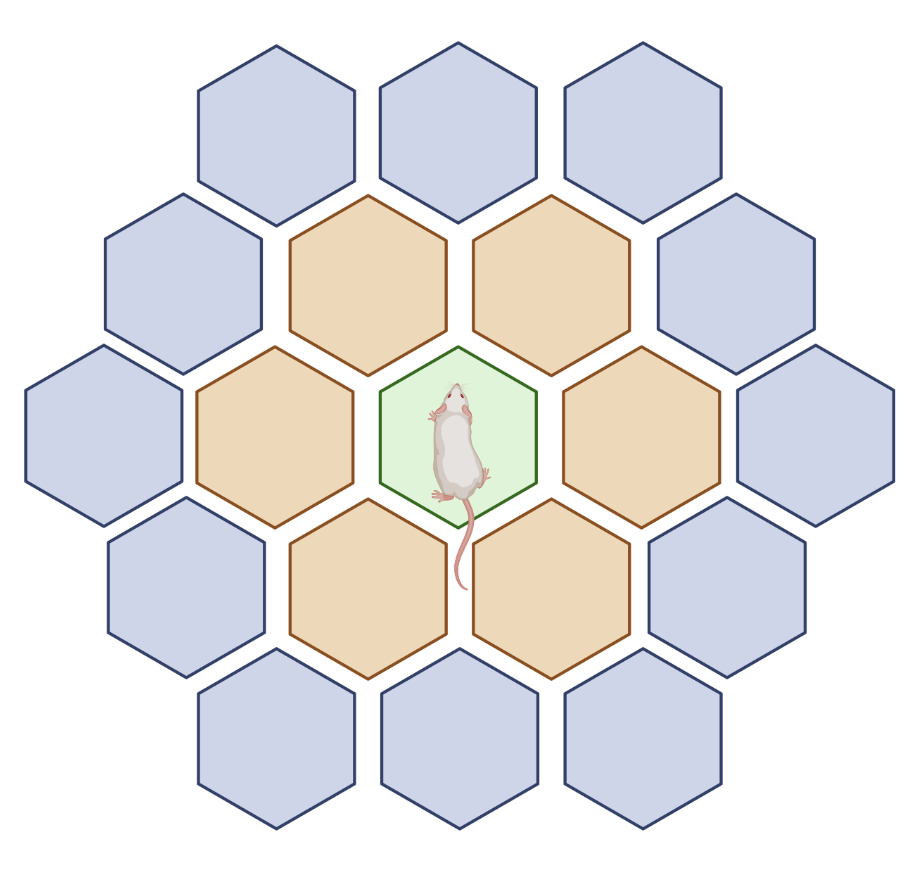
\includegraphics[scale = 0.5 ]{images/outer_rings.png}
    % 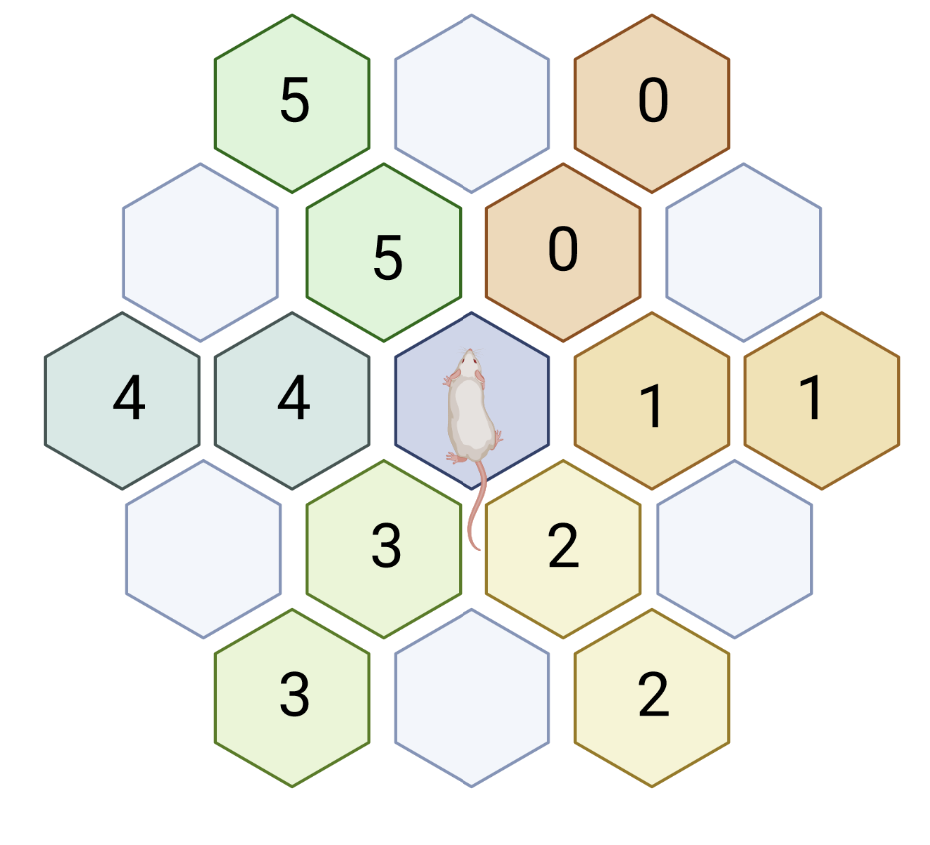
\includegraphics[scale = 0.50]{images/relative_position.png}
    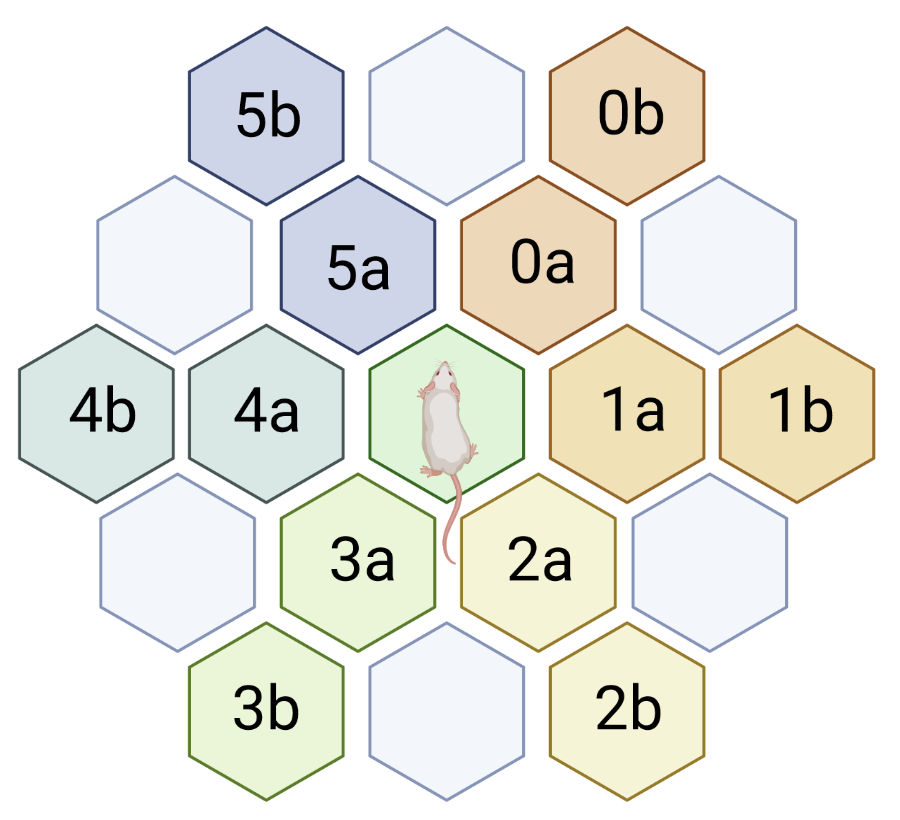
\includegraphics[scale = 0.50]{images/relative_position_mapped.png}
    \caption{This figure shows two important concepts that have been developed: 1. LHS: Inner (\textit{Orange}) and Outer Ring (\textit{Dark Blue}). 2. RHS: Relative Position}
    \label{fig:inner_ring}
\end{figure}


\subsection{\textit{Maze} Class}


% It is important, for handling the boundaries of the maze, defining where robots are allowed to move without letting the path finding algorithm running out of space to complete its moves.

This class defines the boundaries of the maze which the robots move around on. In conjunction with the \textit{Robot} class, it prevents path-finding beyond the boundaries of the maze.

\subsubsection{Coordinate system}

Despite the surface on which the platform move around on being a 2D space, for the task at hand, it can be more intuitive to use a 3D coordinate system to encode the space traversed by the robots. This is because there are six directions the platforms can move out of  at any point in the grid. This can be thought of as three dimensions (where there is a backwards and forwards direction for each of the three dimensions, i.e. positive and negative).

These are the $North-East$ direction, the $East-West$ direction and the $North-West$ direction.

For this program, it has been decided that movement in the: 
\begin{enumerate}
\item $North-East$ direction has been considered to be the $y$ direction
\item $East-West$ direction to be the $z$ direction 
\item $North-West$ direction to be considered $x$ direction
\end{enumerate}

The mathematical embedding of this space is a slice through 3D coordinate system, taken through a diagonal of a cube and what is left is a hexagonal shape (exemplified by Fig. \ref{fig:hexagona_slice_through_cube}), more specifically the plane:
$$x + y + z = 0$$
 This forms a tiled hexagonal surface can be used on which out robots move through.

Based on theses rules the following figure shows the coordinate space that has been used. 
\begin{figure}[h]
    \centering
    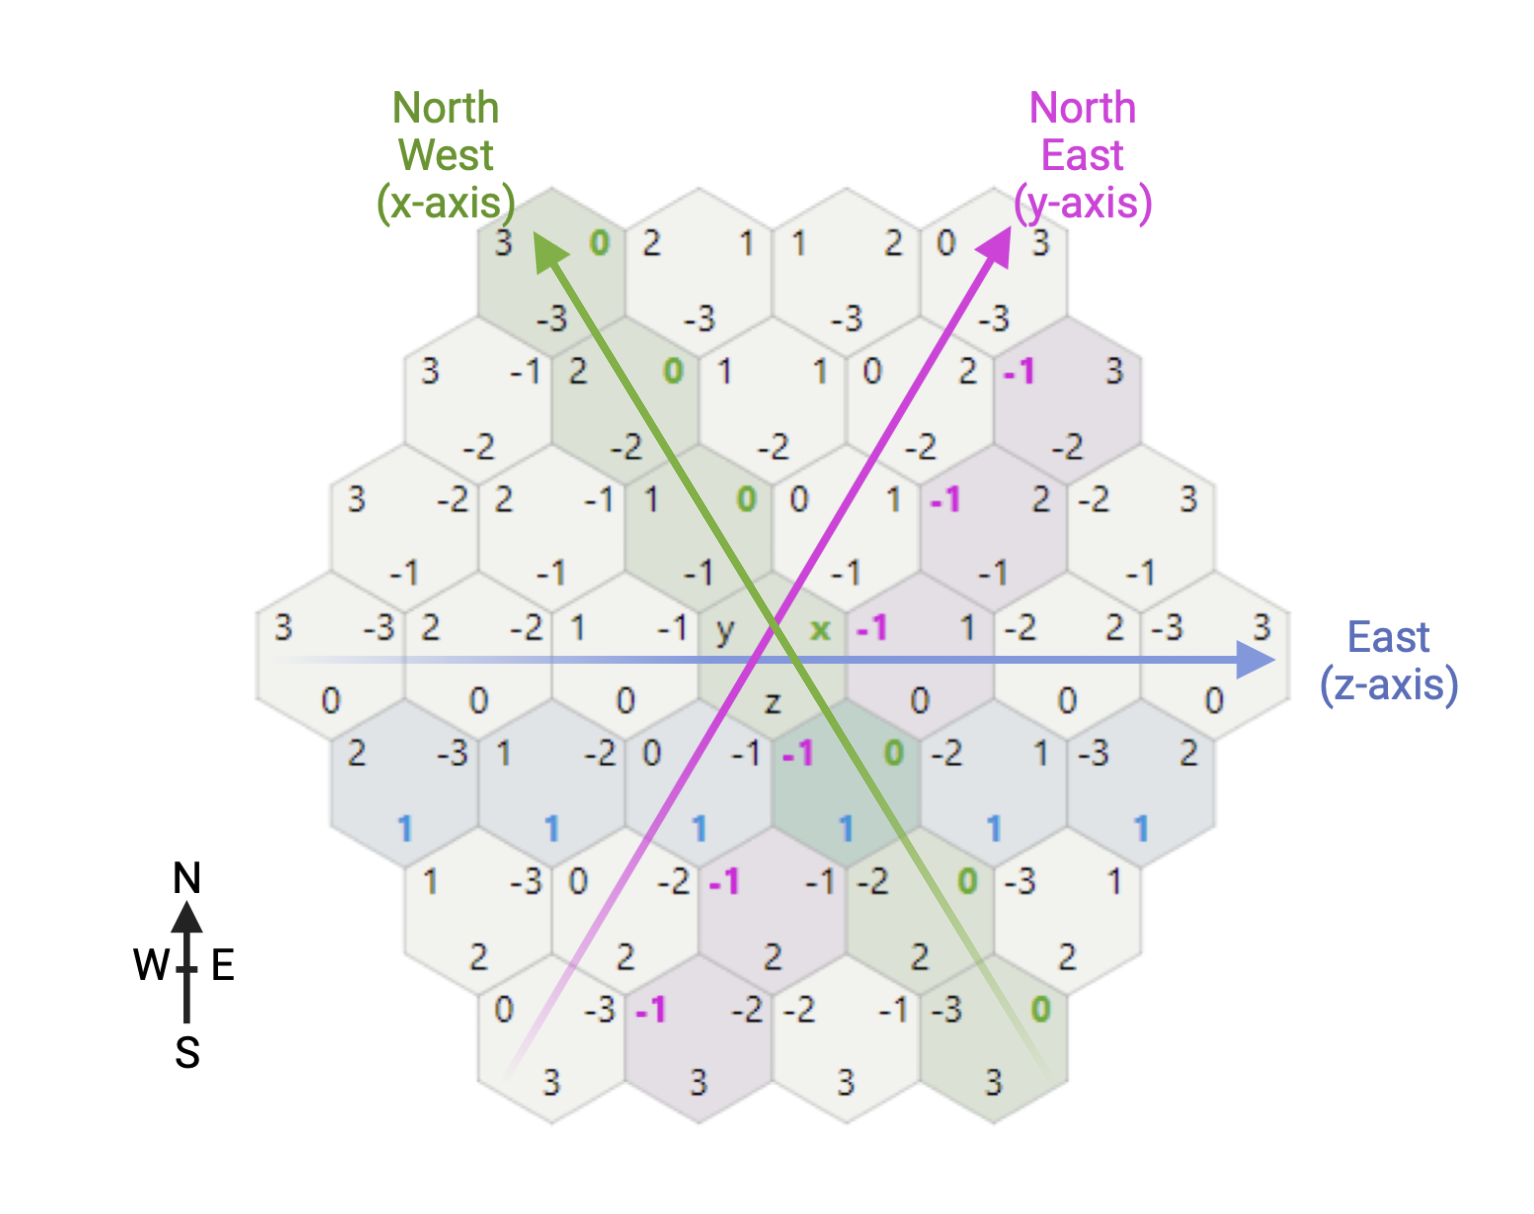
\includegraphics[scale=0.35]{images/hexagon_coordinates_adapted.png}
    \caption{The coordinate system used to encode the 2 dimensional space with a 3D coordinate system. The axis have been defined $North-West$ as $x$, $North-East$ as  $y$ and $East-West$ as $z$. This figure has been adapted from Red Blob Games \cite{patel_2021}}.
    \label{Hexagonal grid coordinates}
\end{figure}

Due to the coordinate system being used, a function has been defined in the \textit{Robot Class} which moves the robot around the coordinate space in a way that ensures the robots position remains defined by Function \ref{function:move_around_hex_grid}.

\pagebreak
\subsection{\textit{Robot} Class}

This is the class which deals with the movement of the robot around the maze in which it is placed. This includes the path-finding algorithm for the robots to move from their initial position to their final position as well as the supporting functions required.

\subsubsection{Overview of the whole path-finding process}

The order of the overall algorithm requires the following steps:

%TC:ignore
\begin{tcolorbox}
\begin{enumerate}
    \item Deciding the order by which the platforms move so that no collisions take place. (Section \ref{section:order_of_operations})
    \item Movement of the platforms away from the animal robot so it can move freely without collision. (Section \ref{section:pre_pathfinding})
    \item Path-finding around the board to their path-finding targets using the Dijkstra Path-finding Algorithm. (Section \ref{section:pathfinding})
    \item Moving into the inner ring of the animal robot so that they are in the new positions and they are consecutive to the animal, allowing the animal to make another decision (to choose another platform) around the maze. (Section \ref{section:post_path_finding})
\end{enumerate}
\end{tcolorbox}
%TC:endignore



\subsubsection{Order of movement of the platforms for the Pre-Path-finding phase}
\label{section:order_of_operations}
Here we discuss the order of operations for the two moving robots must take to prevent them colliding with each other. The algorithm must be robust enough such that no collisions occur for all the possible pairs of positions of the non animal robots around the animal robot. As the IR sensors are only present on the front the robots, a specific method is used to allow the robot to step backwards whilst keeping track of its position (This seen in \ref{fig:stepping_back_method} and implemented with Function \ref{function:stepback_function}).

From Fig \ref{fig:post_decision_states} we see that the platform, which the animal did not choose to move on to, must be the first platform to move backwards away from the robot which used to have the animal on it. If this occurs, the robot is never next to the other two robot meaning it has free range of movement to start the path-finding phase.

After this has occurred, the robot with the animal on it and the robots which used to have the animal on it are left consecutive to each other (so there is limited range of movement between them).

The robot that is left consecutive to the (current) animal robot must always step back into the outer ring of the (current) animal robot. Because we do not know the direction of the unoccupied robot, sometimes this is a move backwards, sometimes forward. This allows the robot free range of movement as it is not consecutive to any other robots.

These two observations imply: (1) that the robot \textbf{\textit{not}} selected must always move first, and (2) the robot that used to be the animal robot must always move second. Both must move without rotation to prevent collision.

It follows that the concept of 'animal robot', 'non-animal robot' and 'non-non-animal robot' can be developed.
%TC:ignore
\begin{tcolorbox}
They are defined in the following way:
\begin{itemize}
    \item \textbf{'Animal Robot' (AR)} is the platform robot that the animal has chosen to move to. This will always be \textbf{stationary} during the path-finding method.
    \item \textbf{'Non-animal Robot'(NAR)} is the platform robot that the animal has come from. This will always be the \textbf{second} robot to move in the path-finding method.
    \item \textbf{'Non-non-animal robot' (NNAR)} is the platform robot that the animal has not chosen, from the two choices. This will always be the \textbf{first} robot to move for the path-finding method.
\end{itemize}
\begin{center}
\textit{From now, the above notation will be used}
\end{center}
\end{tcolorbox}
%TC:endignore
There is a table for reassigning the robots' state, based on their previous and new state, shown in Table \ref{table:change_states_of_robot}).
This negates the requirement for the order of operations having to be calculated from the arrangement and direction of the robots.

\subsubsection{Pre-Pathfinding Phase}
\label{section:pre_pathfinding}

Recall: the animal will be given a decision about which platform to move to. Once this has occurred, the maze will be left with the configurations shown in Figure \ref{fig:post_decision_states} and appendix Figure  \ref{fig:all_post_decision_states}.



\paragraph{1. Non-non Animal Robot (NNAR)}

As demonstrated in Fig. \ref{fig:post_decision_states}, the NNAR must always move backwards away from the NAR. This will ensure that the NNAR is never consecutive to any of the other robots in the system and hence is free to move around.


\begin{figure}[H]
    \centering
    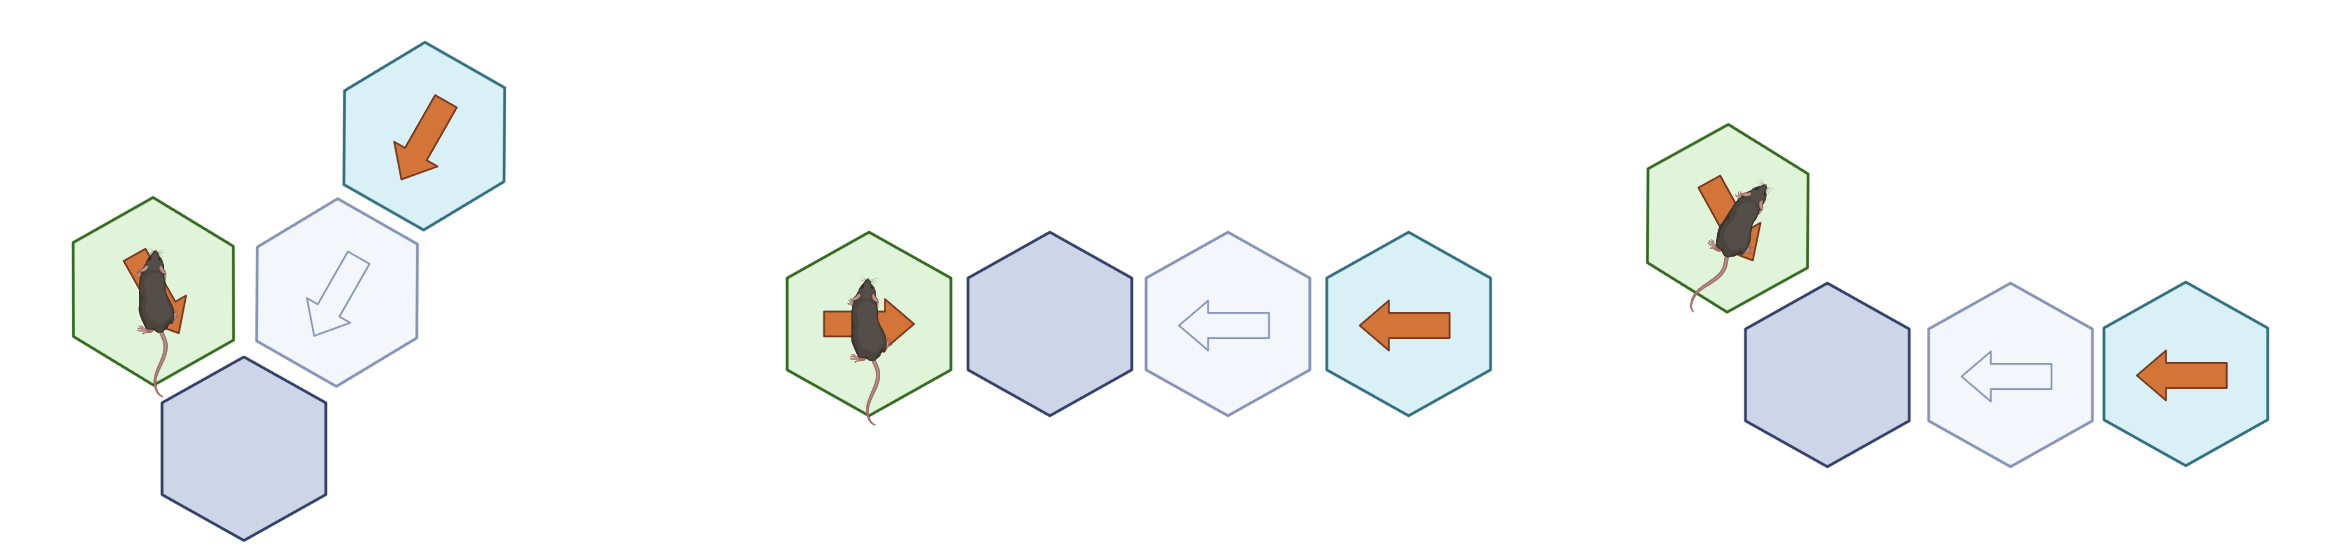
\includegraphics[scale = 0.5]{images/post_decision_state.png}
    \caption{This shows all possible arrangements of the three robots just after the animal has made a decision about which platform to stand on. In this case, the animal started on the blue platform and chose the green platform to stand on afterwards. \\ This demonstrates that the 'non-non-animal robot' must always step one step backwards from the other two robots to make sure there are no other robots that are consecutive to it before it starts path-finding to the outer ring position of the relative position of the path-finding end point.\\ \textbf{Note:} The \textit{dark blue} hexagon is the \textit{Non-animal robot (NAR)}, the \textit{green} hexagon is the \textit{Animal Robot (AR)} and the outlined hexagon is the \textit{Non-non-animal Robot (NNAR)}}
    \label{fig:post_decision_states}
\end{figure}

\paragraph{2. Non-Animal Robot (NAR)}

Demonstrated in Panel D and E in Fig \ref{fig:control_flow_diagram}, the NAR must always move to the outer ring of AR, without turning. Direct movement to another position in the inner ring will result in a collision; see Fig. \ref{fig:collision}. (Note: that this is sometime a step backwards and sometime a step forwards, depending on the rotation of the AR at the time.)

\begin{figure}[H]
    \centering
    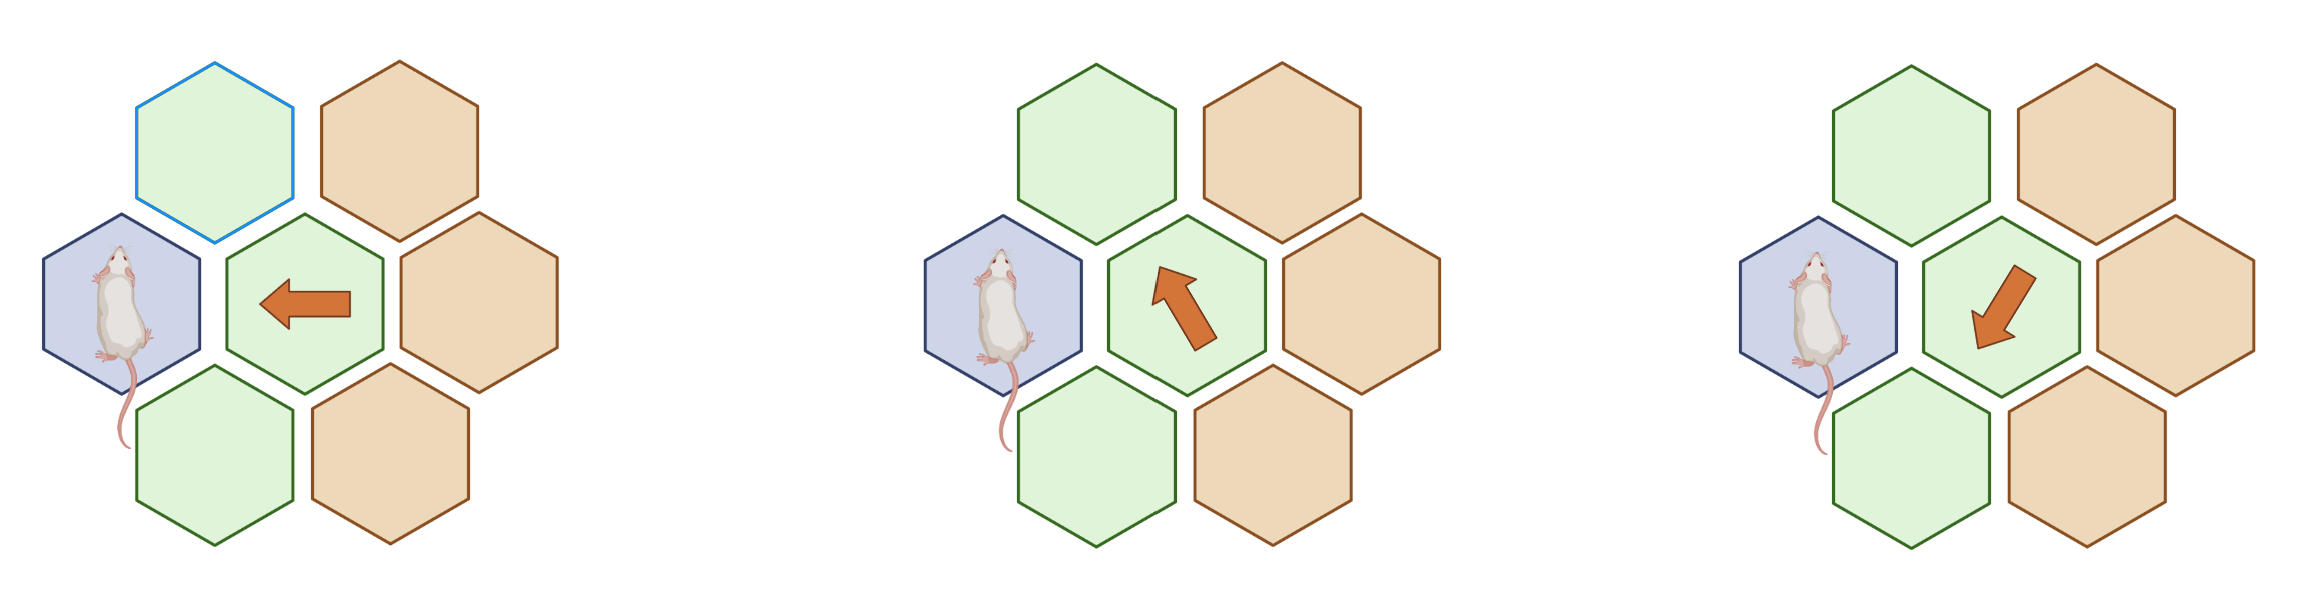
\includegraphics[scale = 0.5]{images/move_to_outer_ring.png}
    \caption{This figure demonstrates that whatever the position of the 'non-animal robot', it must step into the outer ring of the new 'animal robot'. This either means stepping forward once or backwards once, depending on what which was forward is each of these arrangement. Note that is always possible for the 'non-non-animal robot' to move the outer ring.}
    \label{fig:nnar_move_to_outer_ring}
\end{figure}
%TC:ignore
\begin{tcolorbox}
Therefore, in the pre-pathfinding phase of the algorithm:
\begin{enumerate}
    \item NNAR will always move (first) way from the NAR.
    \item NAR will always move (second) into the outer ring of the AR.
\end{enumerate}
\end{tcolorbox}
%TC:endignore
\subsubsection{Pathfinding Phase}
\label{section:pathfinding}

\paragraph{Justification for \textit{networkx} approach} 

A general path-finding algorithm was implemented, instead of a hard-coded solution more specific to the task at hand, because a general path-finding algorithm allows a more versatile version of the program handling more combinations of robot positions without the algorithm failing to find a valid path.

To prevent having to write source code for a general path finding algorithm, a Python library, able to find the shortest path between two points on a network, called \textit{networkx} \cite{networkx} was used instead. This requires the path finding problem presented to be converted into a graph which the library can handle.


The most advanced path-finding algorithm \textif{networkx} supports is the \textit{Dijkstra} path-finding algorithm \cite{dijkstra1959pathfinding}. % Though it is not as efficient or versatile as other path-finding algorithms, such as the A*  path-finding algorithm \cite{A*_pathfinding} \cite{lit_review_pathfinding}, for the size and complexity of network that will be generated for the honeycomb maze, the Dijkstra path-finding algorithm will  suffice. Due to the computational time required to find the path being negliable compared with the time taken for the path found to be executed by the robots.

\paragraph{Implementation of \textit{networkx}}
From the hexagonal grid determined by the \textit{Maze} class, a triangular lattice network of the correct size is generated. This encodes all positions that are possible for the robots are able to move to in the room. A triangular lattice is used as this network connects all nodes (not on the boundary of the grid) to six consecutive nodes, which is the same as the number of adjacent movements possible from each point on the grid.

After the whole movement network was generated, a modified version of the movement network is generated: the \textit{temporary movement network (TMN)} with all moves that would cause collision being removed from the network. When a robot wants to move around the network the positions of the 'non-moving' robots were removed from the \textit{TMN} as well as the \textit{inner-ring} positions for these same robots - as these are the positions that would cause collisions if the robot was moved there.
The \textit{TMN} would be returned to the moving robot, where it would find its path from the \textit{path-finding source} to the \textit{path-finding target}.

\begin{figure}[h]
    \centering 
    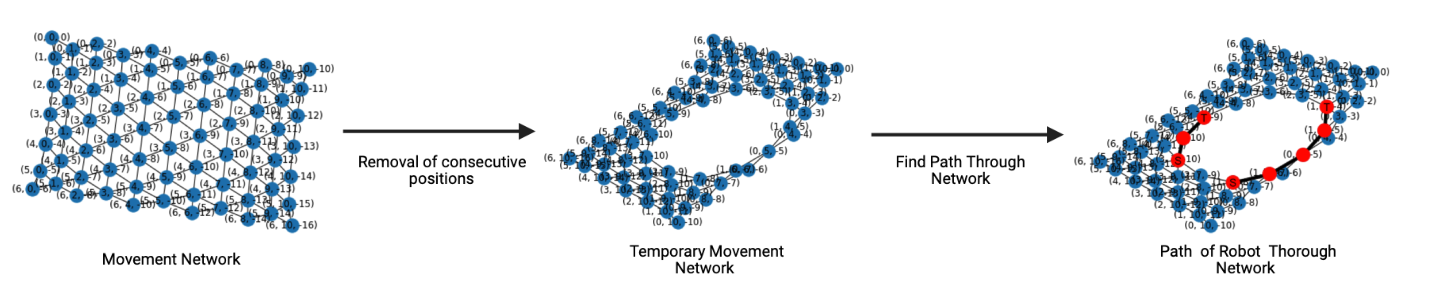
\includegraphics[scale = 0.3]{images/pathfinding_algorithm.png}
    \caption{This shows an example of the network generated by the \textit{networkx} library (LHS image), based on all the possible moves available in the maze. Once the network has been generated, the positions that are impossible to access by the moving robot are removed from the network (RHS image). From this, the shortest path from the \textit{path-finding source} to the \textit{path-finding target} will be found and a list of coordinates that describe the path will be generated and return to the robot. This figure has been generated by the \textit{networkx} package \cite{networkx}.}
    \label{fig:networkx_diagrams}
\end{figure}


\paragraph{Setting Path-finding Targets}
\label{section:pathfinding_targets}

Since the actual source and target of the complete algorithm will always be in the inner ring of the 'non-moving' robots, they are removed from the \textit{TMN}.  Therefore they can not be used as the path-finding source and target for the path-finding algorithm. 

As such, the source and target used are the corresponding outer ring positions of the actual source and target. The way these are calculated, corresponds to the mapping shown Figure \ref{fig:pathfinding_source_target_mapping} from the (blue) inner relative positions to the (pink) outer relative positions.

This allows the moving robot to get to the correct relative position of its target position, however instead of being in the inner ring, where it aims to be, it is in the outer ring.

\begin{figure}[h]
    \centering
    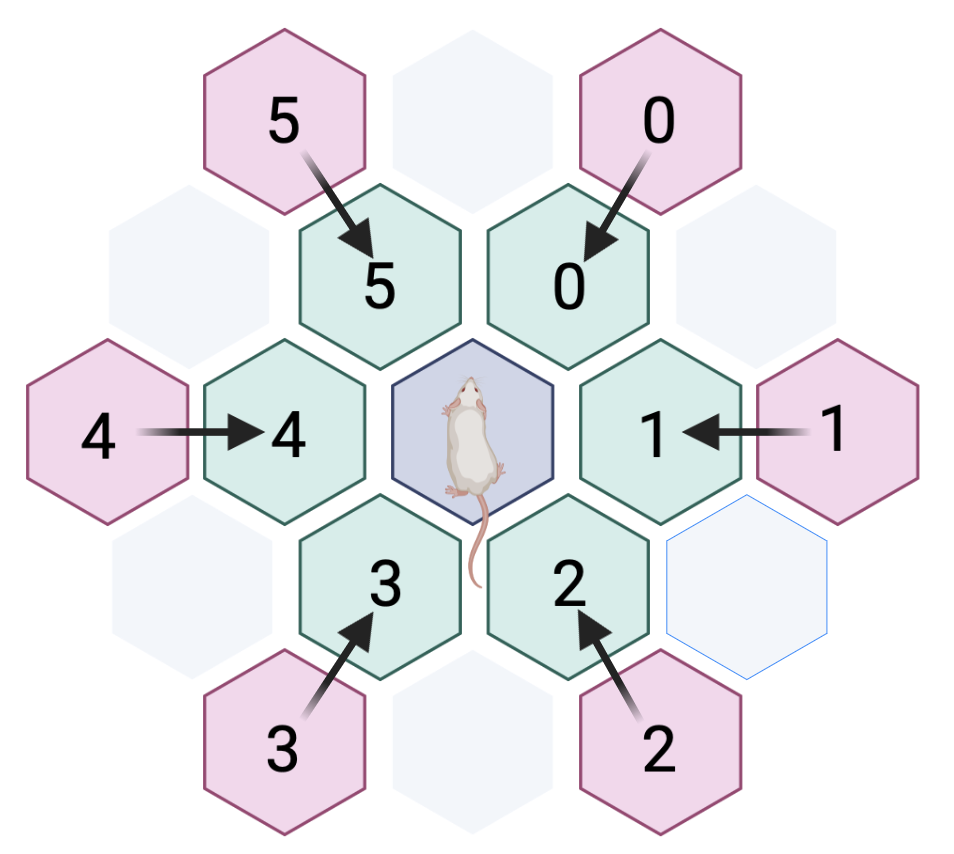
\includegraphics[scale=0.25]{images/move_to_inner_ring_2.png}
    \caption{This figure shows the mapping from the actual source (or target) of the path-finding algorithm (in blue) to the 'path-finding source' or 'path-finding target'  (in pink). This is because \textit{networkx} will not be able to path-find from a position in the network that is not present. As such, the path-finding begins after the 'step back from the NAR' move takes place.\\    In the Post-Path-finding phase (\ref{section:post_path_finding}), both the \textit{NAR} and \textit{NNAR} will be pointing towards to the \textit{AR} when they step forward to get from the outer ring to the inner ring. This means they will \textit{always} be pointing towards the \textit{AR} in their final position thus the start positions shown in panel A of Fig \ref{fig:control_flow_diagram} are all possible valid starting positions that the algorithm must handle.}
    \label{fig:pathfinding_source_target_mapping}
\end{figure}

\subsubsection{Post-Path-finding Phase}
\label{section:post_path_finding}

% As shown in Fig. \ref{fig:nnar_move_to_outer_ring}, after the animal has made its decision, the NNAR must move to the outer ring to make sure that it does not collide with the NAR when executing its path.

The NNAR, (which moves first) will wait until, the NAR has moved to its path-finding source. Once both of the moving robots have reached the end of their path-finding phase, they will both be in the outer ring of their correct relative position.  After this, both NAR and NNAR will move from their \textit{outer ring} position to their corresponding \textit{inner ring} position. They will both be adjacent to the AR providing a choice for which robot the animal would like to occupy in the next. This command is executed at the same time for both robots, making sure that the animal has the same amount of time to consider each platform, reducing bias towards a particular platform.


%\subsubsection{Moving to final position}

% Once the robots has reached their path-finding target, they will be in the in the correct relative position of the required target, however it will be in the outer ring, not the inner ring (as required). Therefore, a move to the inner ring from the outer ring is all that is required to move to their correct position. (In Fig \ref{fig:pathfinding_source_target_mapping}, they will have to move from the (pink) outer ring to the corresponding position (blue) position in the inner ring.

% From combining the ideas from Figure \ref{fig:inner_ring}, it can be seen that the relative positions is a one to one mapping of the six positions on the inner ring to six positions on the outer ring. This becomes very useful because once a robot on on the outer ring position (where the relative position is defined), it can be used to move the robot from the inner ring to the outer ring in a standard way.

% Once the robot has got to the outer ring of the animal robot, where the relative position is defined, all that the robot has to do is to move from the outer ring to the inner ring whilst staying on the line of the same relative position.

% The non animal robot (or non-non animal robot) simply has to point towards the animal robot. Once it has done this, the animal robot simply has to step once forward. Then it will be consecutive to the animal robot. Once this has occurred the animal can make a decision about which robot platform it would like to move  towards.

% Both the \textit{NAR} and \textit{NNAR} will be pointing towards to \textit{AR} when they step forward to get from the outer ring to the inner ring. This means they will \textit{always} be pointing towards the \textit{AR} in their final position. Therefore, the start positions shown in panel A of Fig \ref{fig:control_flow_diagram} are all the valid starting positions that the algorithm must handle.

\\ \\ 

The method of moving the robot to the final position by moving to the inner ring and maintaining relative position, means the robots will always have to turn towards the AR and step forward once as their final move. Thus the orientations shown in panel A of Fig \ref{fig:control_flow_diagram}, showing the non-animal robots' facing the AR, will be the \textit{only} arrangements that occur.

\pagebreak
\subsection{\textit{Animal} Class}

This class defines the position of the animal, which must always be on top of one of the robot platforms. As such,    it will inherit the position of the robot is occupies. The \textit{animal} class is also used to model the decision making that the animal made when testing the program.


\subsubsection{Animal class decision making}

Inside this class of the program is where integration with other computer-vision libraries such as \textit{deeplabcut} \cite{dlc} would occur. It will be updated when the animal moves from one robot to another.

For testing the program, a simple random decision or manual choice - by the user - is made between the two possible choices of platform to move to for testing purposes.

